\chapter{\ifproject%
\ifenglish Project Structure and Methodology\else โครงสร้างและขั้นตอนการทำงาน\fi
\else%
\ifenglish Project Structure\else โครงสร้างของโครงงาน\fi
\fi
}

% ในบทนี้จะกล่าวถึงหลักการ และการออกแบบระบบ

\newcommand{\iptoDomain}[2]{\texttt{#1} $\rightarrow$ \texttt{#2}}

\makeatletter

% \renewcommand\section{\@startsection {section}{1}{\z@}%
%                                    {13.5ex \@plus -1ex \@minus -.2ex}%
%                                    {2.3ex \@plus.2ex}%
%                                    {\normalfont\large\bfseries}}

\makeatother
%\vspace{2ex}
% \titleformat{\section}{\normalfont\bfseries}{\thesection}{1em}{}
% \titlespacing*{\section}{0pt}{10ex}{0pt}

\section{\ifenglish System Architecture\else สถาปัตยกรรมระบบ\fi}

\hspace{1.27cm} \raggedright โครงงานนี้ได้ออกแบบสถาปัตยกรรมของระบบเป็นแบบ Microservices โดยบทนี้จะกล่าวถึงโครงสร้างของระบบทั้งหมด และอธิบายถึงแต่ละส่วนของระบบ โดยระบบจะถูกแบ่งออกเป็นส่วนย่อยๆแต่ละส่วนจะมีหน้าที่และความรับผิดชอบในการทำงานที่แตกต่างกัน 

\begin{figure}[H]
    \centering
    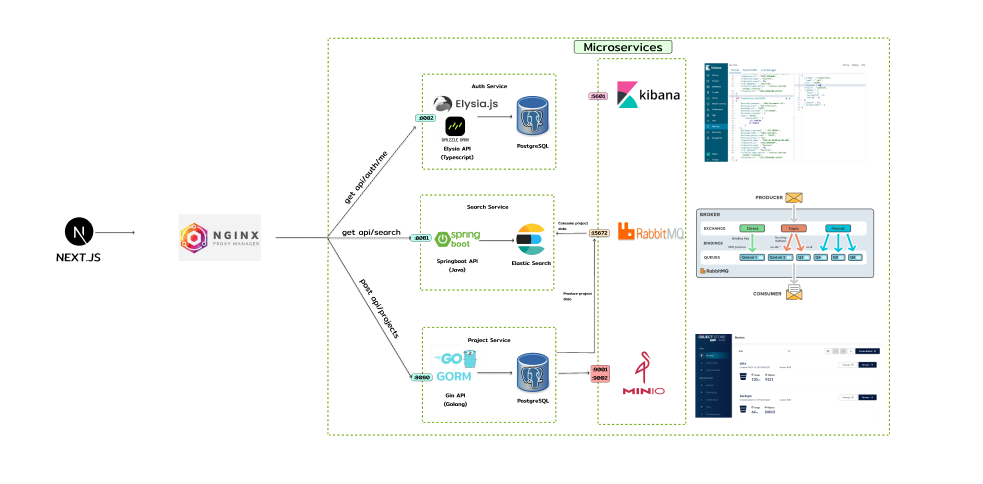
\includegraphics[width=0.8\textwidth]{pictures/architecture.png}
    \caption{รูปภาพแสดงสถาปัตยกรรมของระบบ}
    \label{fig:system_architecture}
  
\end{figure}

จากรูปที่ \ref{fig:system_architecture} แสดงถึงสถาปัตยกรรมของระบบที่ถูกแบ่งออกเป็นส่วนย่อยๆ ดังนี้
\begin{enumerate}
  \item  \textbf{Frontend} ส่วนนี้เป็นส่วนที่ทำหน้าที่ในการแสดงผลของระบบ โดยส่วนนี้จะถูกพัฒนาด้วย Next.js
  \item \textbf{Reverse Proxy} ส่วนนี้เป็นส่วนที่ทำหน้าที่ในการจัดการการเชื่อมต่อระหว่าง Frontend และ Backend โดยส่วนนี้จะถูกพัฒนาด้วย Nginx Proxy Manager(NPM)
  \item \textbf{Backend} ส่วนนี้เป็นส่วนที่ทำหน้าที่ในการจัดการข้อมูลและการทำงานของระบบ โดยส่วนนี้จะถูกแบ่งออกเป็นส่วนย่อยๆ ดังนี้
  \begin{itemize}
    \item \textbf{Auth Service} ส่วนนี้เป็นส่วนที่ทำหน้าที่ในการจัดการข้อมูลของผู้ใช้งาน โดยส่วนนี้จะถูกพัฒนาด้วย Typescript Elysia.js 
    \item \textbf{Project Service} ส่วนนี้เป็นส่วนที่ทำหน้าที่ในการจัดการข้อมูลของโครงงาน โดยส่วนนี้จะถูกพัฒนาด้วย Go Gin 
    \item \textbf{Search Service} ส่วนนี้เป็นส่วนที่ทำหน้าที่ในการค้นหาข้อมูลของโครงงาน โดยส่วนนี้จะถูกพัฒนาด้วย Java Sprint Boot \& Elasticsearch
  \end{itemize}
\end{enumerate}

\section{Frontend}
\hspace{1.27cm} \raggedright ส่วนนี้เป็นส่วนที่ทำหน้าที่ในการแสดงผลของระบบ โดยส่วนนี้จะถูกพัฒนาด้วย Next.js โดยส่วนนี้จะถูกแบ่งออกเป็นส่วนย่อยๆ ดังนี้
\begin{itemize}
  \item \textbf{Dashboard} ส่วนนี้เป็นส่วนที่ทำหน้าที่ในการแสดงผลหน้าแรกของเว็บไซต์หลังทำการ Login เข้าสู่ระบบ
  \begin{figure}[H]
    \centering
    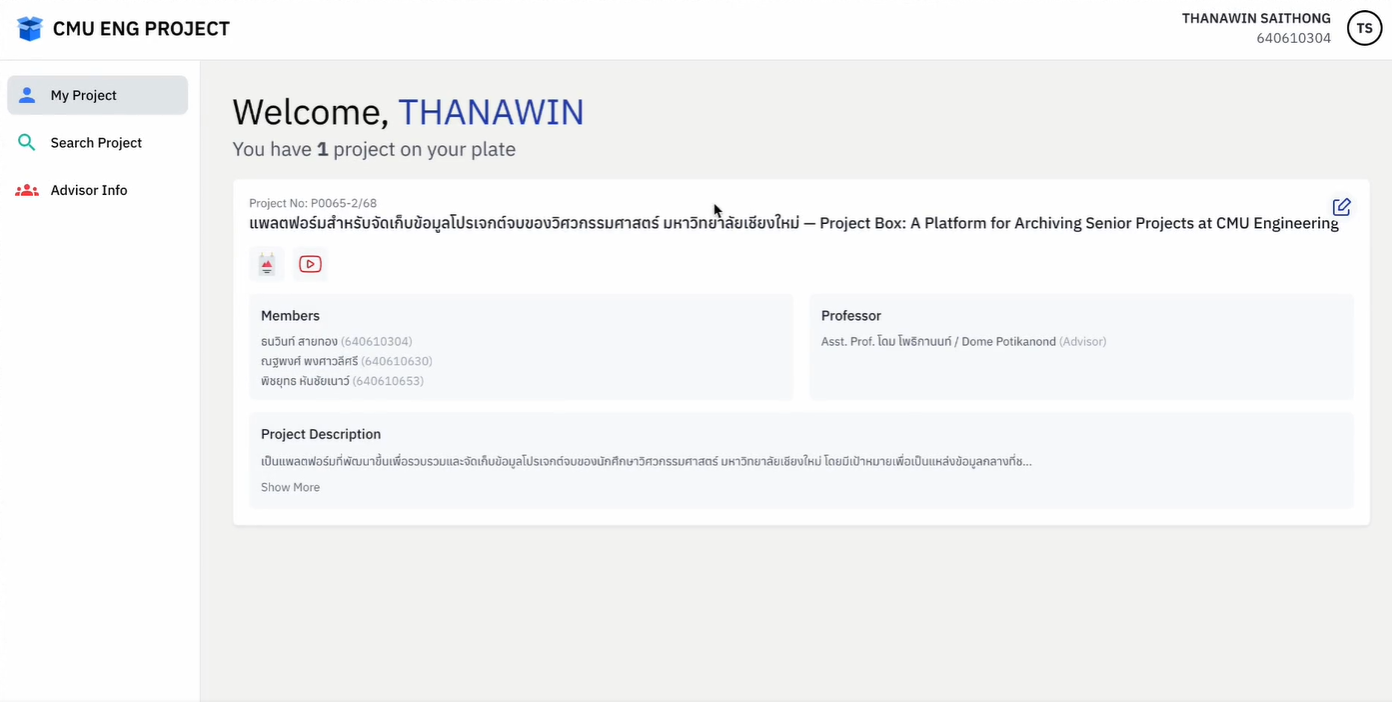
\includegraphics[width=0.8\textwidth]{pictures/project_box/dashboard.png}
    \caption{รูปภาพแสดงหน้าแรกของเว็บไซต์}
    \label{fig:dashboard}
  \end{figure}
  \item \textbf{Advisor Info} ส่วนนี้เป็นส่วนที่ทำหน้าที่ในการแสดงผลหน้าข้อมูลของอาจารย์ที่ปรึกษา
  \begin{figure}[H]
    \centering
    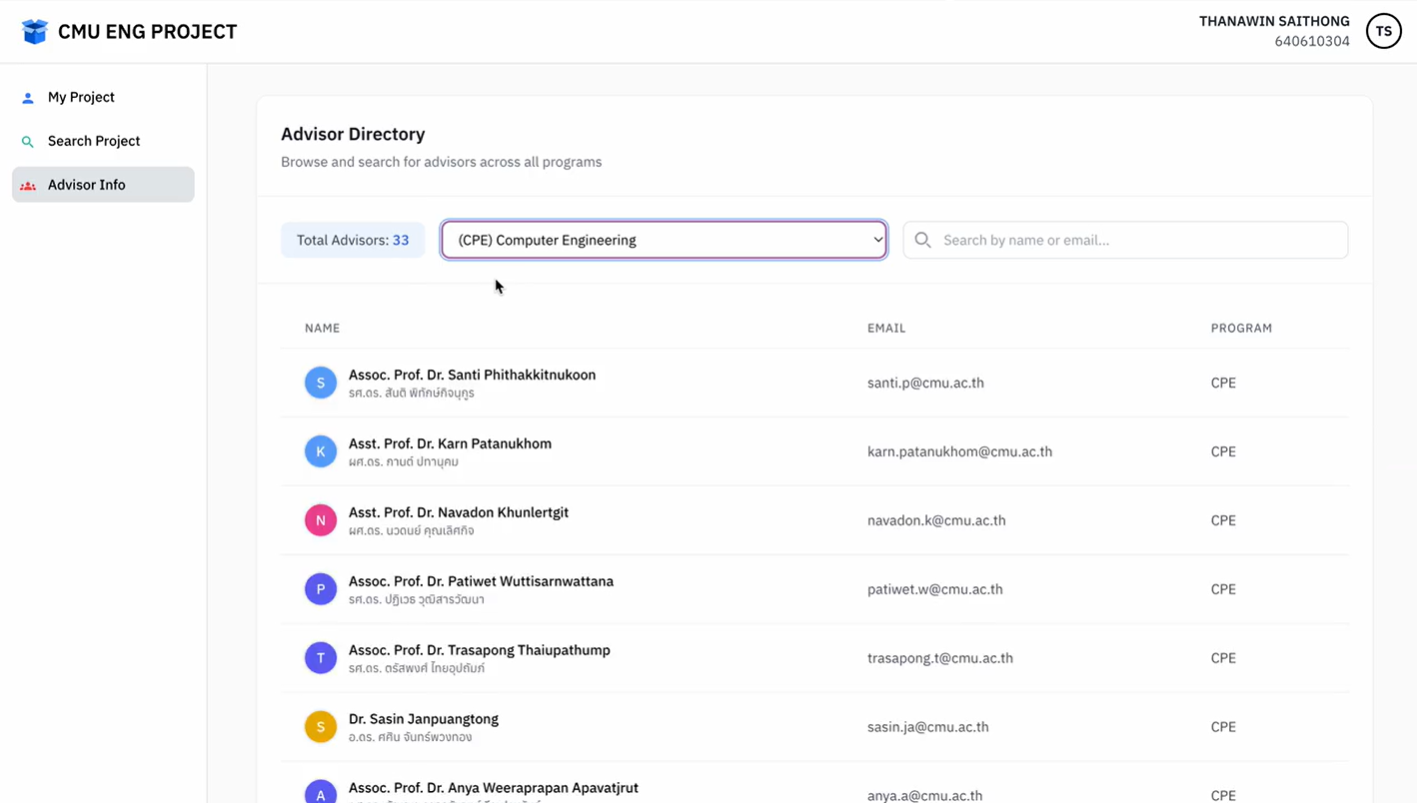
\includegraphics[width=0.8\textwidth]{pictures/project_box/advisor_info.png}
    \caption{รูปภาพแสดงหน้าข้อมูลของอาจารย์ที่ปรึกษา}
    \label{fig:advisor_info}
  \end{figure}
  \item \textbf{Search} ส่วนนี้เป็นส่วนที่ทำหน้าที่ในการแสดงผลหน้าค้นหา สามารถเลือกประเภทของการค้นหาได้
  \begin{figure}[H]
    \centering
    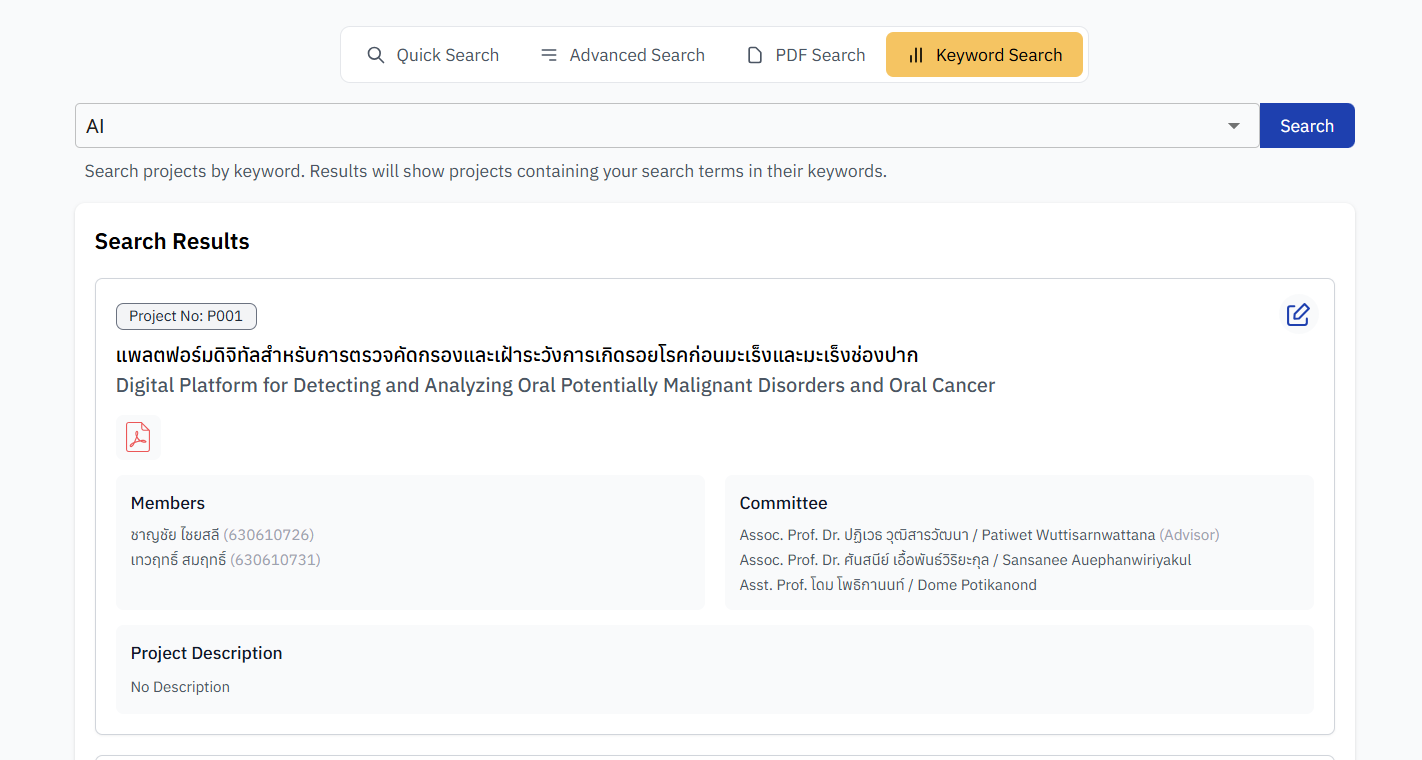
\includegraphics[width=0.8\textwidth]{pictures/project_box/keyword_search.png}
    
  \end{figure}
  \item \textbf{Manage Student} ส่วนนี้คือหน้าที่ใช้ในการจัดการข้อมูลของนักศึกษาหรือเพิ่มโครงงานเข้าไปในระบบ
  \begin{figure}[H]
    \centering
    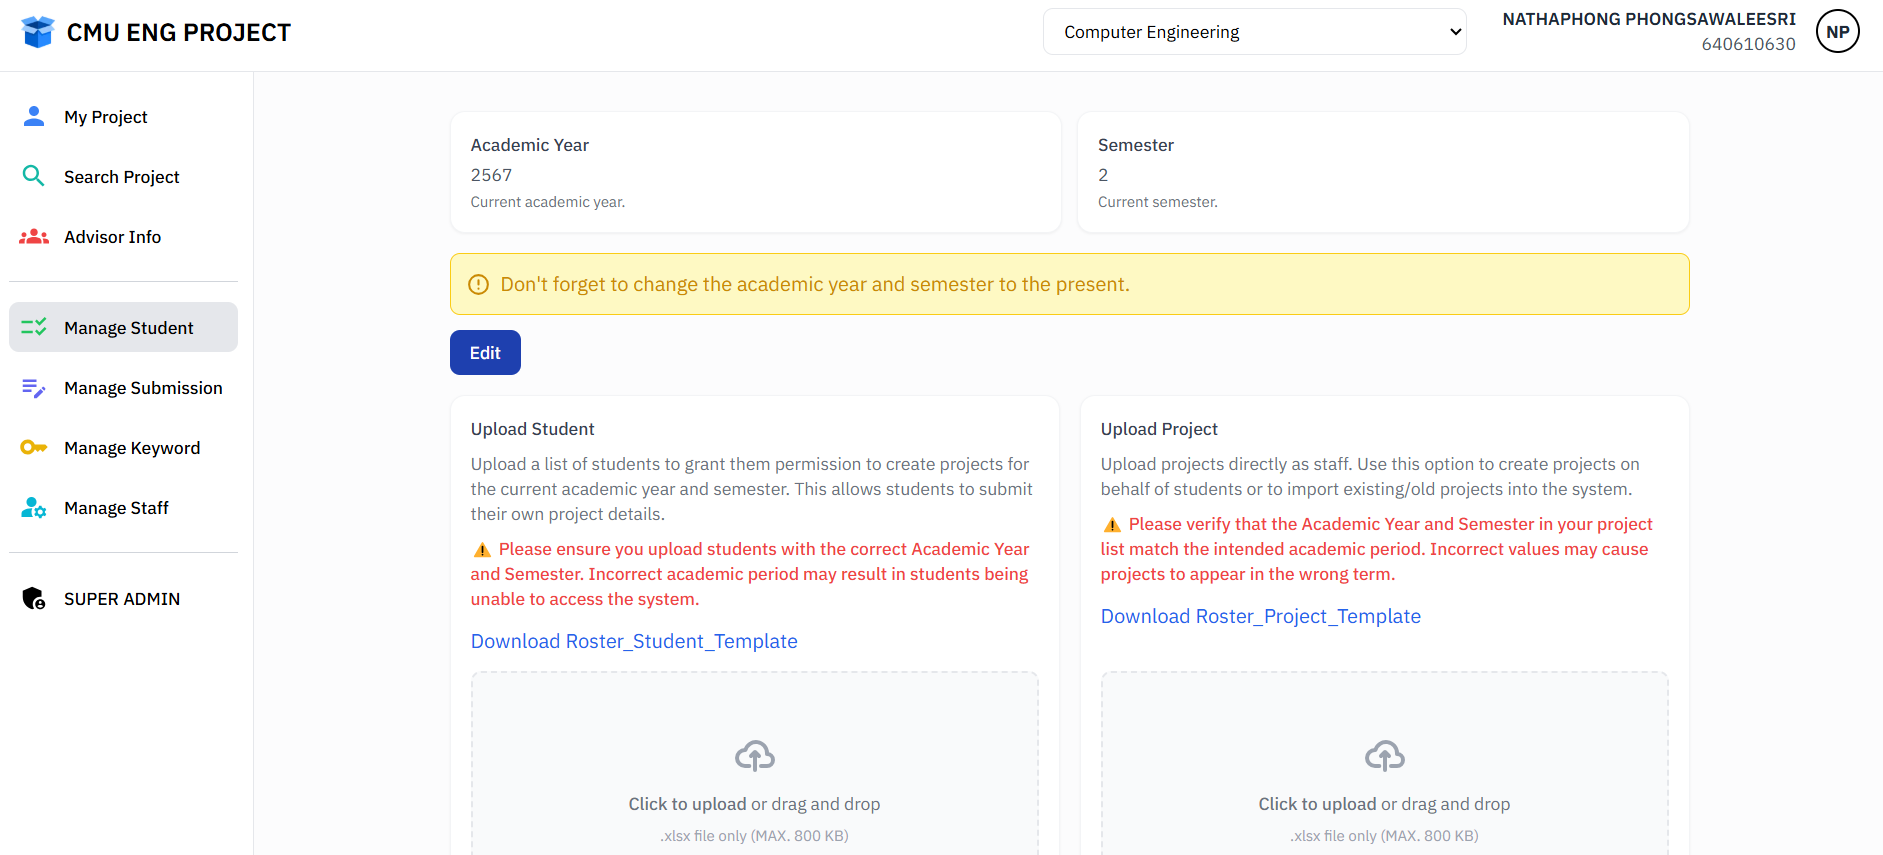
\includegraphics[width=0.8\textwidth]{pictures/project_box/manage_student.png}
    \caption{รูปภาพแสดงหน้าจัดการข้อมูลของนักศึกษา}
    \label{fig:manage_student}
    
  \end{figure}

  \item \textbf{Manage Submission} ส่วนนี้เป็นส่วนที่ทำหน้าที่ในการจัดการข้อมูลของการส่งงานของนักศึกษา
  \begin{figure}[H]
    \centering
    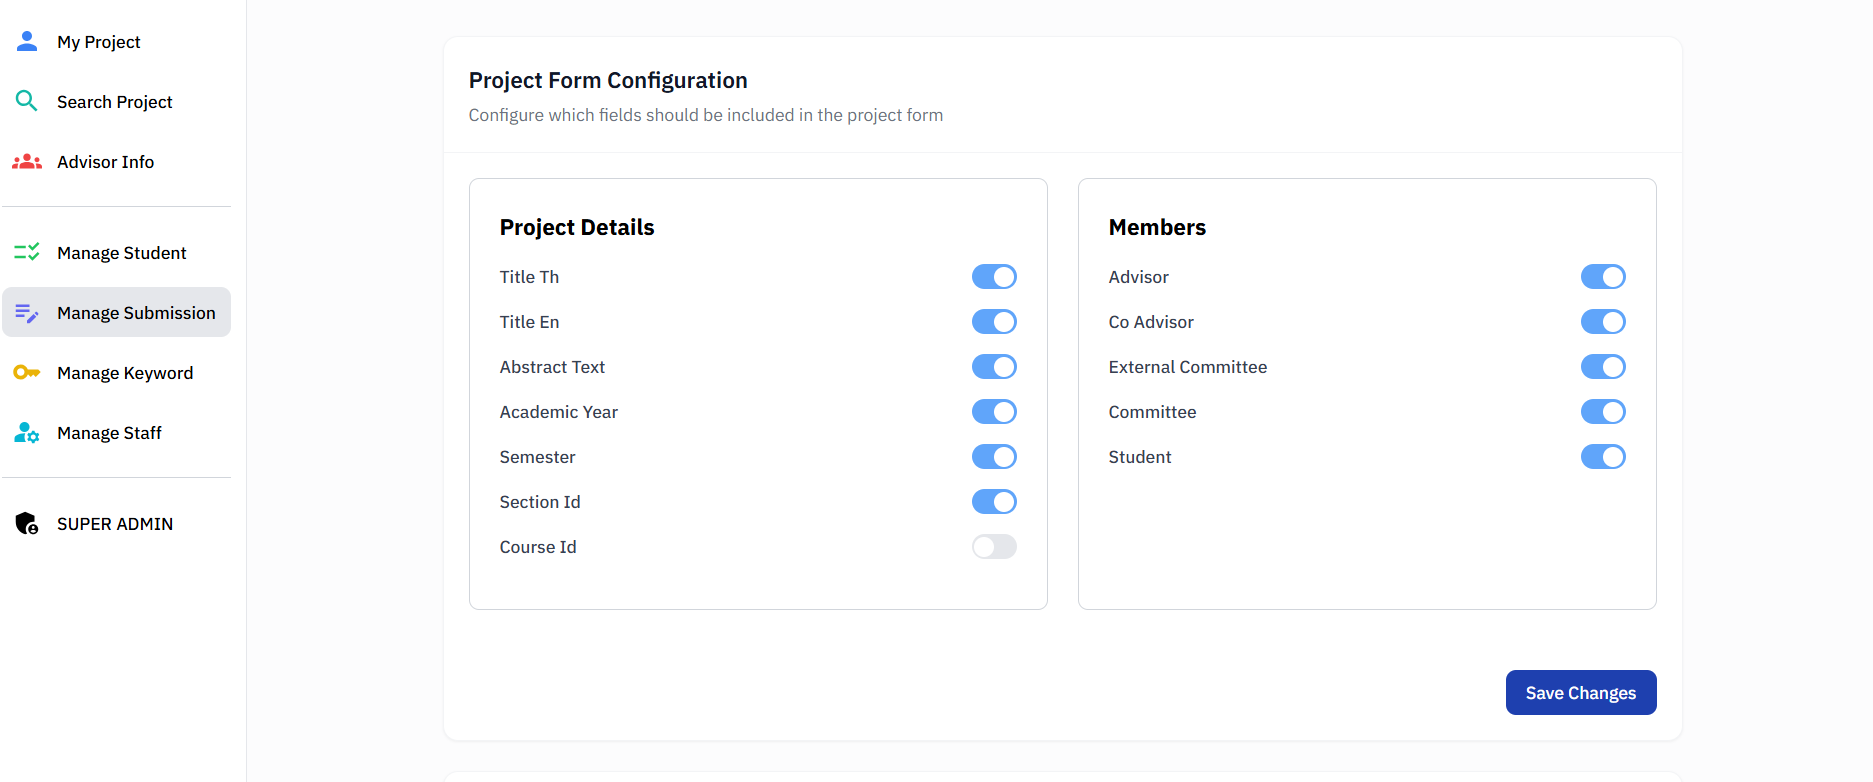
\includegraphics[width=0.8\textwidth]{pictures/project_box/manage_submission.png}
    \caption{รูปภาพแสดงหน้าจัดการข้อมูลของการส่งงานของนักศึกษา}
    \label{fig:manage_submission}
\end{figure}

\item \textbf{Manage Keyword} ส่วนนี้เป็นส่วนที่ทำหน้าที่ในการจัดการข้อมูลของ Keyword ที่ใช้ในการค้นหา
\begin{figure}[H]
  \centering
  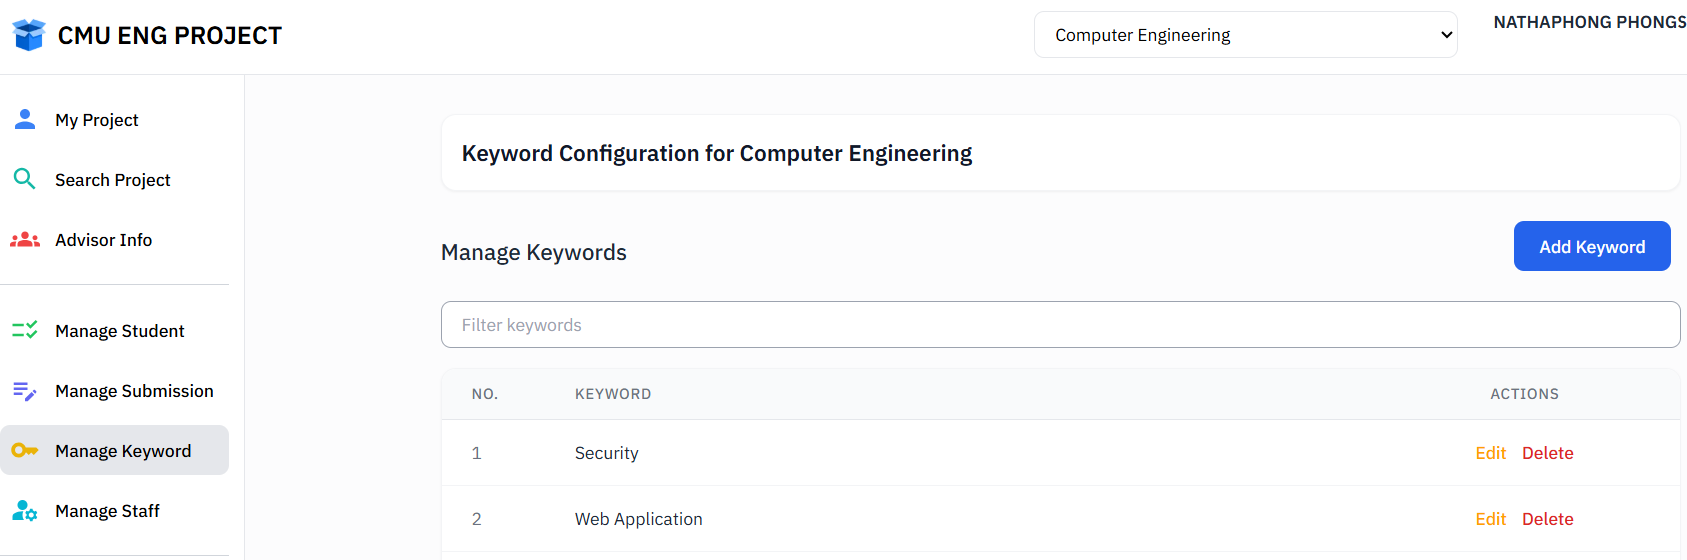
\includegraphics[width=0.8\textwidth]{pictures/project_box/manage_keyword.png}
  \caption{รูปภาพแสดงหน้าจัดการข้อมูลของ Keyword ที่ใช้ในการค้นหา}
  \label{fig:manage_keyword}
\end{figure}
\item \textbf{Manage Staff} ส่วนนี้เป็นส่วนที่ทำหน้าที่ในการจัดการข้อมูลของบุคลากร
\begin{figure}[H]
  \centering
  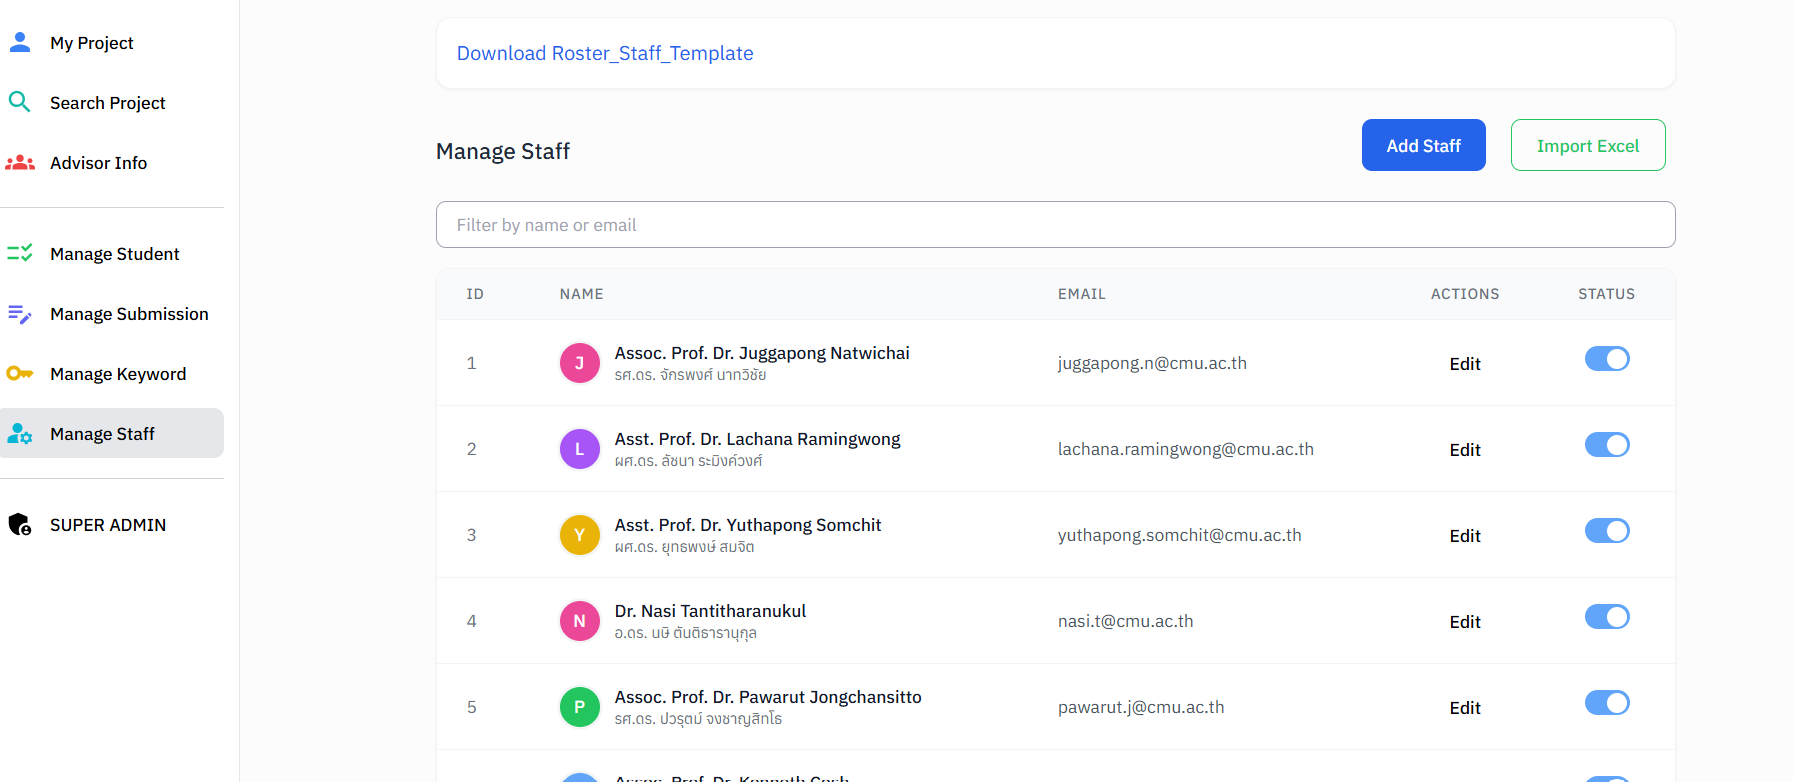
\includegraphics[width=0.8\textwidth]{pictures/project_box/manage_staff.png}
  \caption{รูปภาพแสดงหน้าจัดการข้อมูลของบุคลากร}
  \label{fig:manage_staff}
\end{figure}
\item \textbf{Super Admin} ส่วนนี้เป็นส่วนที่ทำหน้าที่ในการจัดการข้อมูลของผู้ดูแลระบบ
\begin{figure}[H]
  \centering
  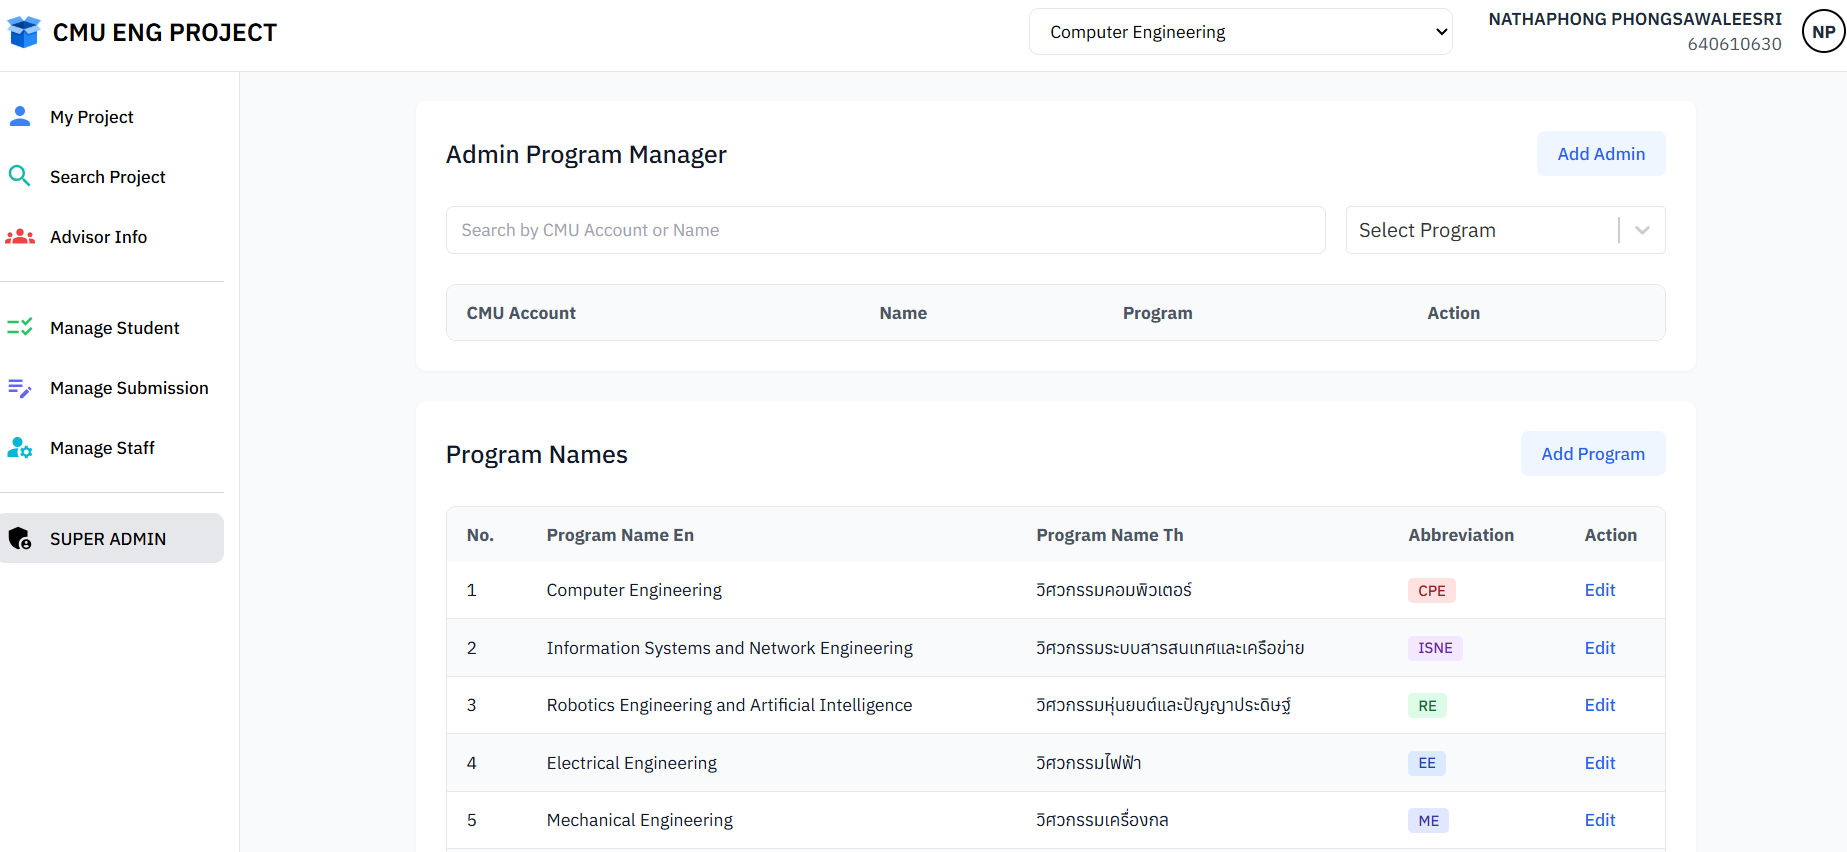
\includegraphics[width=0.8\textwidth]{pictures/project_box/super_admin.png}
  \caption{รูปภาพแสดงหน้าจัดการข้อมูลของผู้ดูแลระบบ}
  \label{fig:super_admin}
  
\end{figure}
\end{itemize}

\section{Reverse Proxy}
\hspace{1.27cm} \raggedright ส่วนนี้เป็นส่วนที่ทำหน้าที่ในการจัดการการเชื่อมต่อระหว่าง Frontend และ Backend โดยส่วนนี้จะถูกพัฒนาด้วย Nginx Proxy Manager(NPM)\cite{npm} มีหน้าที่คือ
การแปลง ip addres ของ server ให้เป็น domain name ยกตัวอย่างเช่น แปลง IP Addres
\iptoDomain{139.59.117.147:8080}{domainname.com}
\enskip โดยส่วนนี้จะทำให้เราสามารถเข้าถึงเว็บไซต์ผ่าน domainname.com ได้ และยังสามารถจัดการการเชื่อมต่อระหว่าง Frontend และ Backend ได้อีกด้วย
\begin{figure}[H]
  \centering
  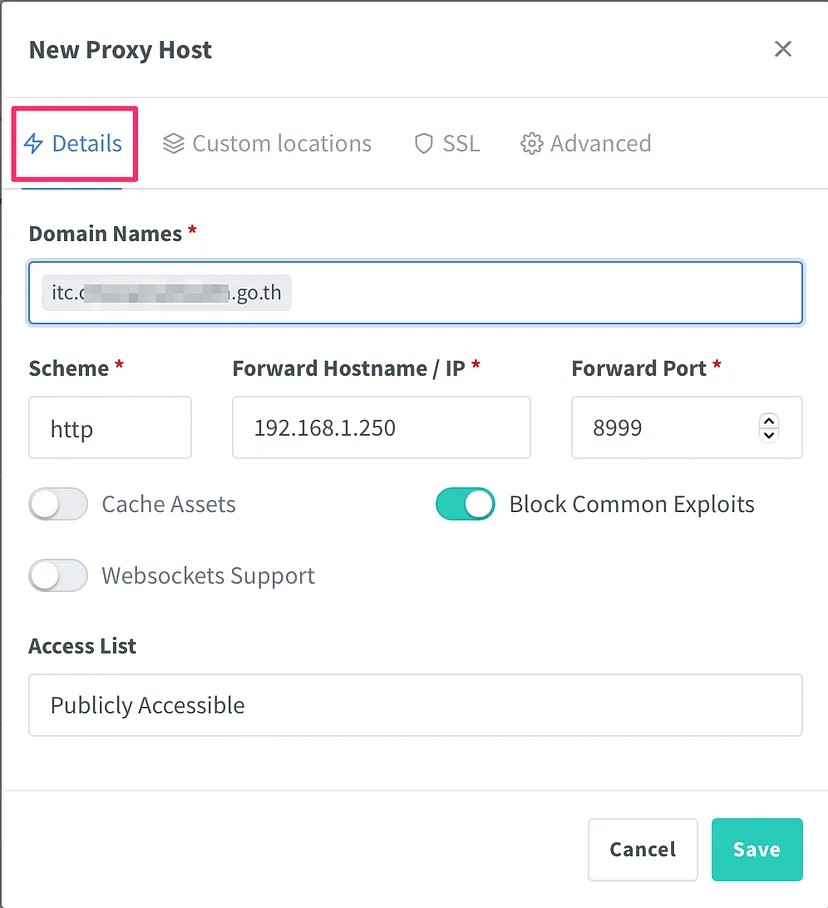
\includegraphics[width=0.8\textwidth]{pictures/npm1.png}
  \caption{รูปภาพแสดงการทแปลง IP ของ Nginx Reverse Proxy}
  \label{fig:reverse_proxy}
\end{figure}
\hspace{ 1.27cm}อีก feature นึงที่สำคัญของ Nginx Reverse Proxy คือการจัดการ SSL Certificate โดย Reverse Proxy จะทำหน้าที่ในการจัดการ SSL Certificate ให้กับเว็บไซต์ ซึ่งจะทำให้เว็บไซต์มีความปลอดภัยมากขึ้น และยังสามารถใช้งานได้ทั้งบน http และ https อีกด้วย
\begin{figure}
  \centering
  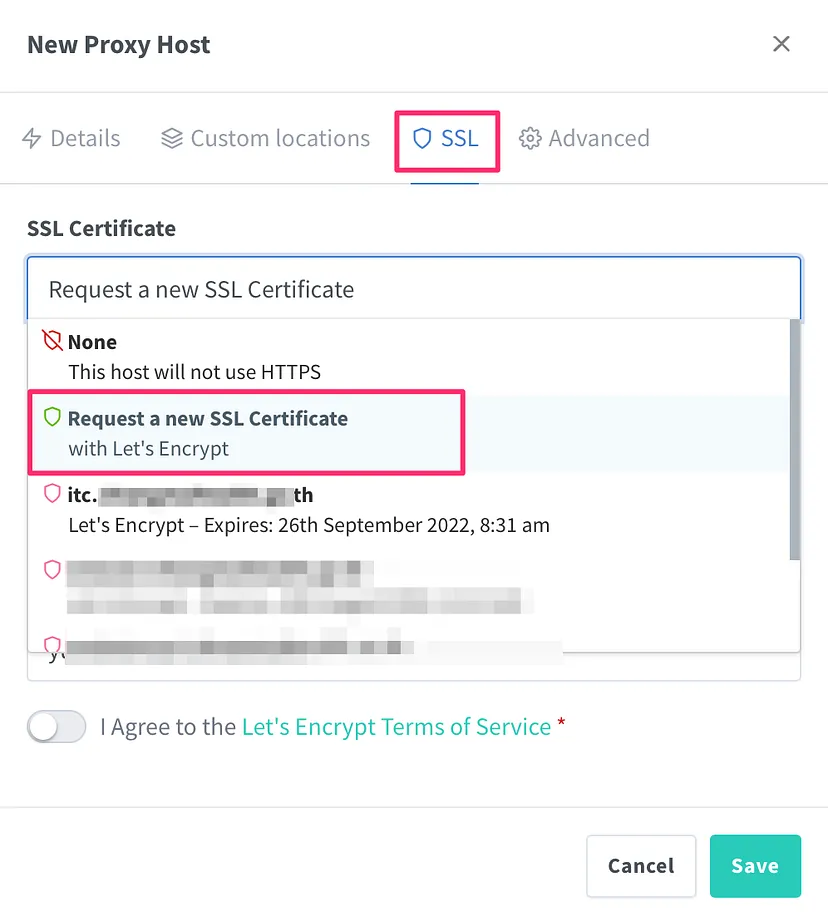
\includegraphics[width=0.8\textwidth]{pictures/encrpt.png}
  \caption{รูปภาพแสดงการจัดการ SSL Certificate ของ Nginx Reverse Proxy}
  \label{fig:reverse_proxy_ssl}
\end{figure}
\section{Backend}
\hspace{1.27cm} \raggedright ส่วนนี้เป็นส่วนที่ทำหน้าที่ในการจัดการข้อมูลและการทำงานของระบบ โดยส่วนนี้จะถูกแบ่งออกเป็นส่วนย่อยๆ ดังนี้
\subsection{Auth Service} 
\hspace{1.27cm} \raggedright ส่วนนี้เป็นส่วนที่ทำหน้าที่ในการจัดการข้อมูลของผู้ใช้งาน โดยส่วนนี้จะถูกพัฒนาด้วย Typescript Elysia.js โดยส่วนนี้จะมีหน้าที่คือ
จัดการข้อมูลของผู้ใช้งานทำหน้าที่ในการเข้าสู่ระบบ และจัดการสิทธิ์ของผู้ใช้งาน(Role) โดยมีการใช้งาน Oauth2 ในการจัดการการเข้าสู่ระบบ และมีการใช้งาน JWT เพื่อสร้าง Token ส่งกลับไปยัง Frontend
\subsubsection{Database Schema}
\begin{figure}[H]
  \centering
  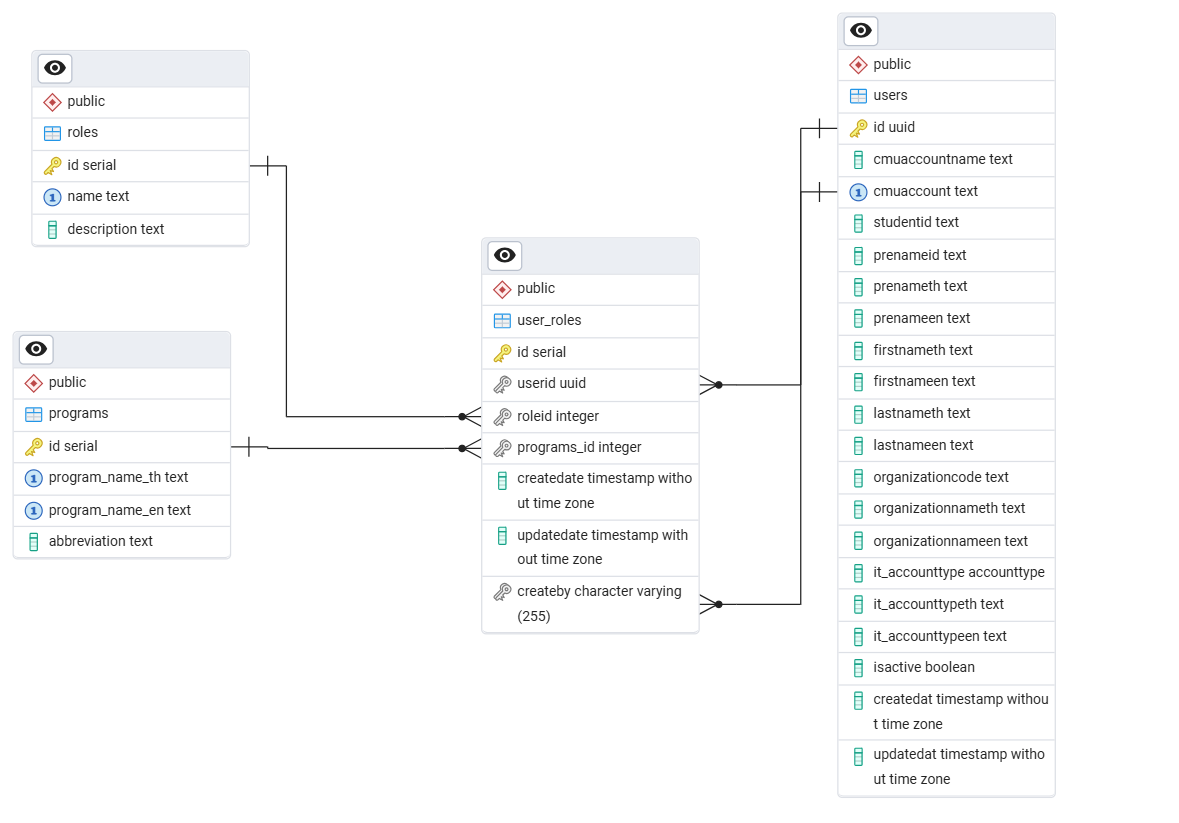
\includegraphics[width=0.8\textwidth]{pictures/auth_db.png}
  \caption{รูปภาพแสดง Database Schema ของ Auth Service}
  \label{fig:auth_service}
\end{figure}
\textbf{\ifenglish Database Schema\else โครงสร้างของฐานข้อมูล\fi}
\begin{itemize}
  \item \textbf{users} ตารางนี้จะเป็นตารางที่เก็บข้อมูลของผู้ใช้งาน 
  \item \textbf{roles} ตารางนี้จะเป็นตารางที่เก็บข้อมูลของตำแหน่งของผู้ใช้งาน
  \item \textbf{programs} ตารางนี้จะเป็นตารางที่เก็บข้อมูลของโปรแกรมหรือหลักศสูตรที่มีอยู่ในระบบ
  \item \textbf{user\_roles} ตารางนี้จะแสดงถึงความสัมพันธ์ของผู้ใช้งานกับตำแหน่งของผู้ใช้งานในโปรแกรมหรือหลักสูตรนั้นๆ
\end{itemize}
\subsection{Project Service}
\subsection{Search Service}

